% =========================================================
\section{Experimental Design}
\label{sec:experiments}
% =========================================================

\subsection{Temporal O\&M Benchmark}
\label{sec:dataset}

We construct TEF-RAG v6 Semantic Benchmark v1 for controlled evaluation of temporal evidence retrieval in dynamic O\&M scenarios. The dataset is constrained by public-source background information and constructed with AI assistance; it is not derived from real power-station fault logs and is not a real O\&M dataset manually annotated by domain experts. Public product documents and research datasets are used primarily to constrain cell type, typical physical ranges, and sampling background, whereas specific O\&M event processes, diagnostic changes, procedure contexts, and query tasks are produced through a controlled synthetic construction process. This design allows us to deliberately introduce late-arriving records, supersession, cross-source complementary evidence, multi-episode ambiguity, and persistent uncertainty, and to compare how different retrieval methods handle these factors.

The overall benchmark construction process is illustrated in Fig.~\ref{fig:benchmark_design}. Public sources first provide constraints on the physical and sampling background. Synthetic O\&M event chains are then constructed under these constraints, from which retrievable evidence records and different task queries are derived. For each query, we separately construct a reference evidence flow for retrieval and a structured reference answer for generation.

\begin{figure*}[t]
    \centering
    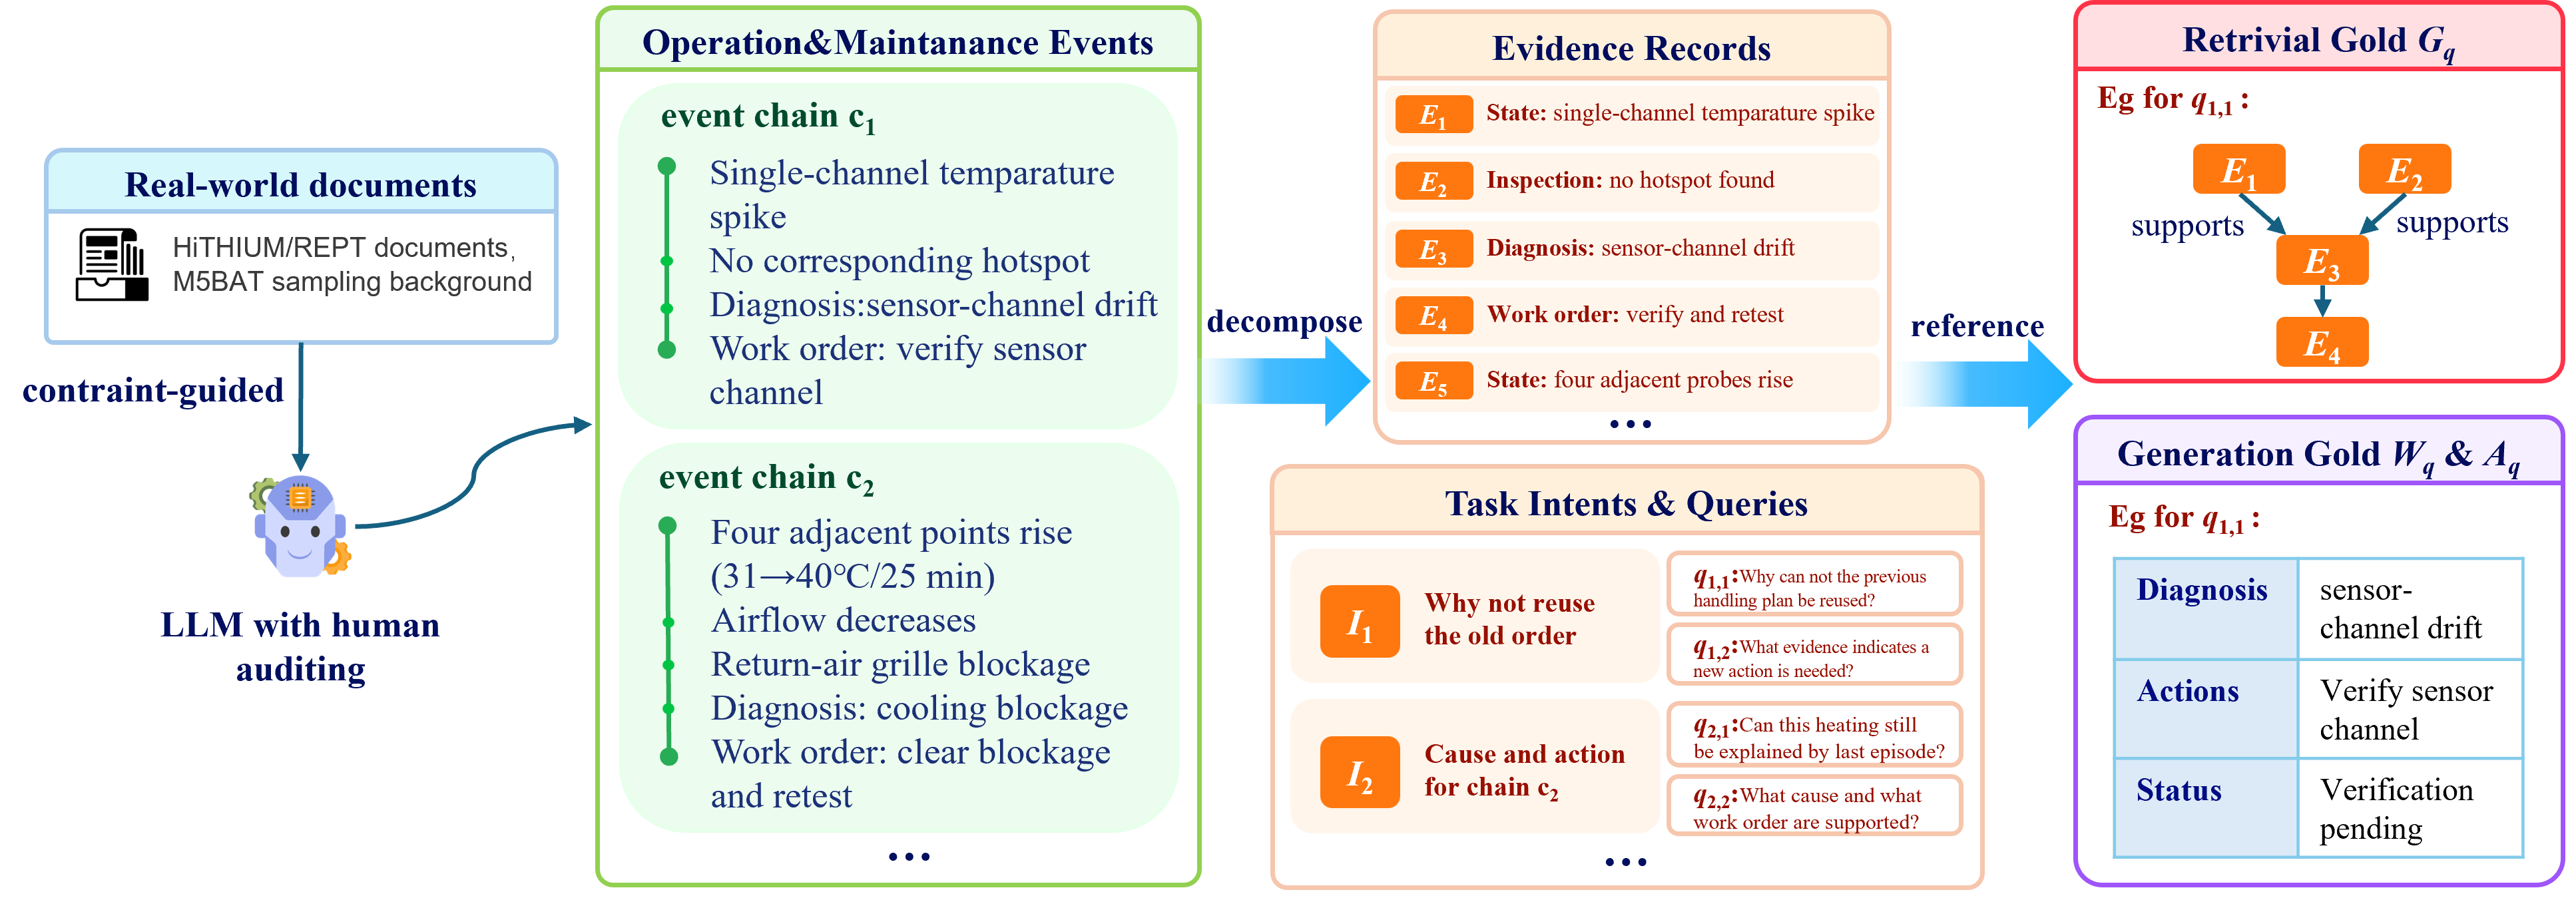
\includegraphics[width=0.98\textwidth]{figures/benchmark_design.png}
    \caption{Construction pipeline and example for TEF-RAG v6 Semantic Benchmark v1. Public sources constrain the equipment and data background; an O\&M event chain $c$ is then constructed and used to derive evidence records $e_i$, task intents $I_j$, and queries $q_{j,p}$. Retrieval reference evidence flows and structured generation reference answers are subsequently created for each query to support retrieval and downstream generation evaluation.}
    \label{fig:benchmark_design}
\end{figure*}

The data organization is summarized in Table~\ref{tab:dataset_structure}. Each event chain represents a complete O\&M process and consists of multiple retrievable evidence records. For each event chain, we construct several distinct task intents, and each intent is expressed through two queries with the same meaning but different wording.

For each query, we further provide a set of reference annotations that specifies which key information must be retrieved to complete the task and what relations those pieces of evidence should satisfy. The evaluation therefore does not require retrieving one uniquely specified text. Instead, it tests whether the retrieved set contains sufficient information and whether the evidence can jointly form a complete task-support process.

\begin{table}[t]
\caption{Data hierarchy of the benchmark.}
\label{tab:dataset_structure}
\centering
\small
\begin{tabular}{@{}p{0.24\columnwidth}p{0.69\columnwidth}@{}}
\toprule
Level & Meaning \\
\midrule
Chain & A complete O\&M event process \\
Evidence & An atomic retrievable record with event time and availability time \\
Intent & A distinct O\&M information need defined on the same chain \\
Query & A differently worded query expressing the same intent \\
Gold flow & Key evidence requirements and their relation constraints \\
\bottomrule
\end{tabular}
\end{table}

The full benchmark contains 400 O\&M event chains, 3,888 evidence records, 1,200 task intents, and 2,400 queries, involving 100 target assets. Development, validation, and test sets are split at the complete event-chain level. All queries derived from the same event chain appear in only one data split, preventing the same event content from appearing in both training and test data through different phrasings.

The benchmark further contains two difficulty layers, each with 200 event chains. The Realistic Distribution Set mainly covers more common temporal and O\&M combinations, while the Temporal-Hard Challenge Set deliberately increases difficult cases involving late-arriving evidence, supersession, multi-episode ambiguity, cross-source complementary evidence, and persistent uncertainty.

\begin{table*}[t]
\caption{Scale and split of TEF-RAG v6 Semantic Benchmark v1.}
\label{tab:dataset_stats}
\centering
\small
\begin{tabular}{lrrrr}
\toprule
Statistic & Development & Validation & Test & Total \\
\midrule
Authored chains & 240 & 80 & 80 & 400 \\
Primary intents & 720 & 240 & 240 & 1200 \\
Query rows & 1440 & 480 & 480 & 2400 \\
Evidence records & 2335 & 779 & 774 & 3888 \\
\bottomrule
\end{tabular}
\end{table*}

Public sources are used only to constrain cell type, typical operating ranges, and temporal sampling background, including energy-storage cell documents from HiTHIUM and REPT BATTERO and the RWTH M5BAT dataset~\cite{hithium2023v11,hithium2024v33,rept2025,rwth2026m5bat}. These sources are not used to define synthetic fault frequencies, station-level thresholds, or specific maintenance causal narratives in our benchmark.

\subsection{Structured Generation Evaluation}

To test whether improvements in retrieval quality further improve downstream generation, we construct structured generation reference answers (generation gold) on the same set of O\&M event chains. These reference answers are generated with AI assistance and finalized through multiple rounds of review, consistency checking, and disagreement adjudication.

Each task intent corresponds to one structured reference answer. Because the two queries under the same intent differ only in wording while requiring the same diagnosis, action, and verification information, they share the same reference answer. The development, validation, and test sets therefore contain 720, 240, and 240 structured reference answers, corresponding to 1,440, 480, and 480 queries, respectively. Each output has two parts: a standardized \texttt{work\_order} and an \texttt{action\_plan}. The work order describes the diagnosis, recommended actions, applicable procedure, verification/uncertainty status, and evidence citations; the action plan consists of atomic actions and their dependencies.

\subsection{Baselines}
\label{sec:baselines}

To ensure that comparisons reflect only differences in retrieval strategy, all methods first operate on the same legal evidence snapshot. We retain only records for the target asset satisfying
$t_e(e)\le t_q$ and $t_a(e)\le t_q$, and apply the same version-validity, withdrawal-status, and model-applicability constraints to procedure evidence. We compare five methods under this shared setup, with a final retrieval budget of at most five evidence records for every method.

\textbf{BM25.}
We use standard BM25 as the lexical retrieval baseline~\cite{robertson2009bm25}. A separate index is built over the legal evidence snapshot for each query, with fixed parameters $k_1=1.5$ and $b=0.75$, and the five highest-scoring evidence records are returned directly.

\textbf{BGE Reranker.}
We first retrieve the Top-30 candidates using the same BM25 setup and then use \texttt{BAAI/bge-reranker-v2-m3} to rescore each $(\text{query},\text{evidence})$ text pair~\cite{chen2024bgem3}. The top five records under the reranking score are selected. This baseline tests whether a general-purpose semantic reranker can compensate for the limitations of purely lexical retrieval.

\textbf{Temporal-BM25.}
This baseline explicitly adds temporal matching to BM25 relevance. Its ranking score is
\begin{equation}
s_{\mathrm{TBM25}}(e,q)
=
\lambda\,\widetilde{s}_{\mathrm{BM25}}(e,q)
+
(1-\lambda)\,s_{\mathrm{time}}(e,q),
\end{equation}
where $\widetilde{s}_{\mathrm{BM25}}$ is the normalized BM25 score and $s_{\mathrm{time}}$ measures the match between the evidence event time and the target time implied by expressions such as years, time intervals, before/after, and current/latest in the query. For queries without explicit temporal intent, the temporal term is set to a constant, preserving the original BM25 ranking. Before final test evaluation, we compare $\lambda\in\{0.25,0.50,0.75\}$ during parameter selection and freeze the best value, $\lambda=0.25$, for subsequent evaluation.

\textbf{TA-RAG.}
We adopt the Time-Aware RAG method of Lau et al.~\cite{lau2025tarag}. The method first decomposes a query into its topic and target time range, then restricts candidate documents using temporal-interval filtering and performs semantic retrieval and BGE reranking within the temporal candidate set. To adapt TA-RAG to our discrete O\&M events, the \texttt{event\_time} of each evidence record is mapped to a one-second half-open interval, and relative temporal expressions in a query are interpreted with $t_q$ as the reference time. In addition, the TA-RAG index is built only over the legal evidence snapshot for the current query, preventing future records from affecting retrieval. Except for replacing the LLM backend with a fixed DeepSeek model, the temporal decomposition, interval filtering, Nomic embedding, FAISS retrieval, and BGE reranking pipeline follows the public implementation.

\textbf{TEF-RAG.}
Our method further applies learned evidence-pair screening, query-conditioned relation-graph construction, and nonlinear set-level ranking over the same legal evidence snapshot, and returns the candidate set with the highest overall evidence-flow score.

\subsection{Evaluation Metrics}
\label{sec:metrics}

\textbf{Retrieval.}
Recall@5 and nDCG@5 measure conventional retrieval relevance. Complete@5 measures whether the retrieved set contains all categories of key evidence required to complete the task. FlowComplete@5 further checks whether those records can form correct and mutually consistent evidence relations, thereby constituting a complete Temporal Evidence Flow.

\textbf{Generation.}
We report four primary metrics in the main text: Field Macro F1 (strict), Action F1, Citation F1, and Plan EM (strict). They measure strict matching of key work-order fields, normalized actions, claim--evidence citations, and the complete action plan, respectively.

\subsection{Ablation Setup}

To analyze which components contribute to the final performance, we conduct four frozen ablations on 480 validation queries: removing learned pair proposal, removing relation-graph-derived set features, removing hard-negative mining, and removing the nonlinear set ranker. The full model and all variants share the same Top-30 search pool, pair budget, relation prompt/threshold, and candidate-set definition. The graph-feature ablation removes only relation-graph-derived set features and retrains the same RankNet; the hard-negative ablation keeps only the first training round; and the nonlinear-ranker ablation falls back to the frozen Stage-3A selector. No new hyperparameter search is performed for these ablations, and no new test predictions are run or test gold accessed. The ablations are therefore used only for component attribution and not to reselect the final test configuration.

\subsection{Experimental Controls}

Development, validation, and final test data are strictly separated for retrieval. All model selection and training use only development/validation information, and the final test is evaluated once after the configuration is frozen. For generation comparison, all methods use the same downstream generator, prompt/schema, and decoding settings; only the retrieved evidence supplied to the generator changes. This design attributes downstream generation differences to retrieval-context quality rather than generator configuration.
